\documentclass[11pt]{report}
\usepackage{graphicx,wrapfig}
\usepackage[pdftex,
            pdfauthor={Jeffrey Yoo Warren},
            pdftitle={Grassroots Mapping: a toolkit for participatory and activist cartography},
            pdfsubject={Participatory Cartography},
            pdfkeywords={Cartography},
            pdfproducer={Latex with hyperref},
            pdfcreator={pdflatex,colorlinks}]{hyperref}
\title{Grassroots Mapping: a toolkit for participatory and activist cartography}
\author{Jeffrey Warren}
\date{May 7, 2010}

\begin{document}
\maketitle

\chapter{Chapter 1}

\section{In This First Section}

This is the first section.

\subsection{We Have This First Subsection}

This is the first subsection.

The foundations of the rigorous study of \emph{analysis} were laid in the nineteenth century, notably by the mathematicians Cauchy and Weierstrass. Central to the study of this subject are the formal definitions of \emph{limits} and \emph{continuity}.

\begin{figure}[h]
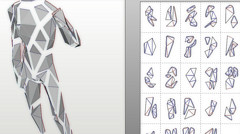
\includegraphics[scale=0.75]{images/test.jpg}
\end{figure}

The foundations of the rigorous study of \emph{analysis} were laid in the nineteenth century, notably by the mathematicians Cauchy and Weierstrass. Central to the study of this subject are the formal definitions of \emph{limits} and \emph{continuity}.

\begin{wrapfigure}{r}{40mm}
  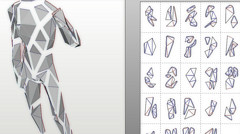
\includegraphics[scale=0.75]{images/test.jpg}
  \caption{The Toucan}
\end{wrapfigure}

\end{document}
